\documentclass[border=6pt]{standalone}
\usepackage{tikz}
\usetikzlibrary{arrows.meta,positioning,fit,backgrounds,calc}
\usepackage[T1]{fontenc}
\usepackage{lmodern}
\begin{document}
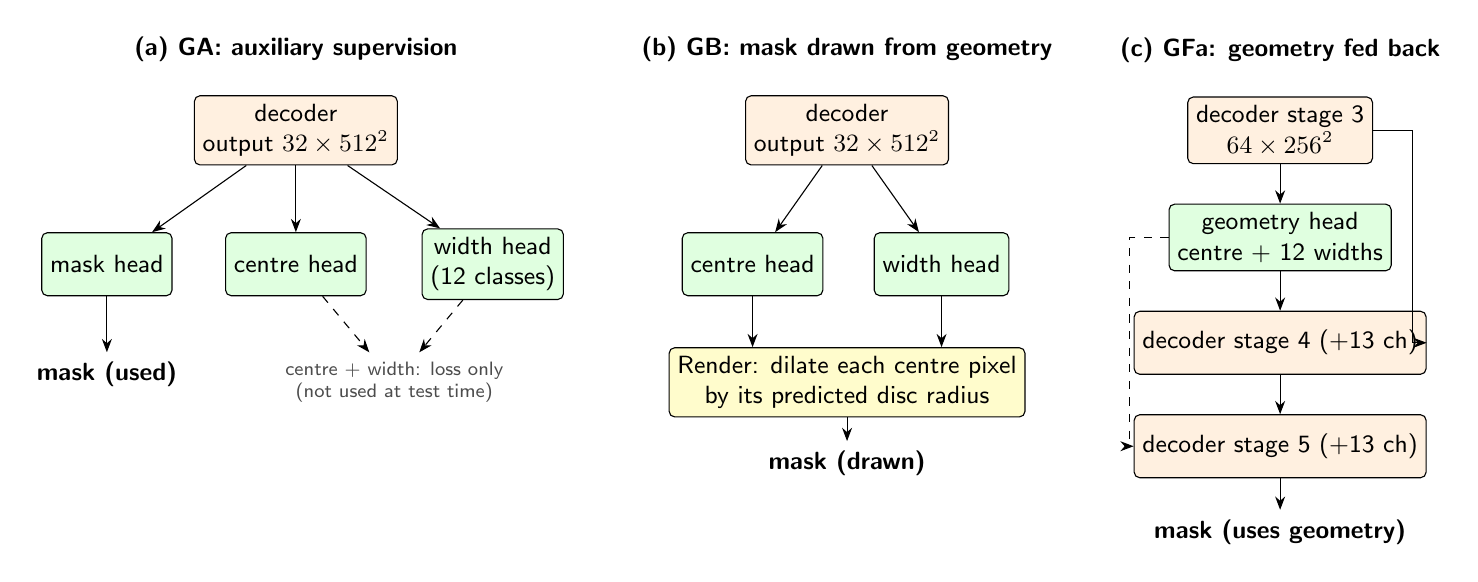
\begin{tikzpicture}[
  font=\sffamily\small, >=Stealth, node distance=4mm and 5mm,
  d/.style={draw, rounded corners=2pt, align=center, inner sep=3pt, fill=orange!12, minimum height=8mm},
  h/.style={draw, rounded corners=2pt, align=center, inner sep=3pt, fill=green!12, minimum height=8mm},
  r/.style={draw, rounded corners=2pt, align=center, inner sep=3pt, fill=yellow!20, minimum height=8mm},
  o/.style={align=center, font=\sffamily\small\bfseries},
  l/.style={align=center, font=\sffamily\scriptsize, text=gray!60!black},
  title/.style={font=\sffamily\bfseries\small, anchor=south}]
% GA
\node[d] (da) at (0,0) {decoder\\output $32\times512^2$};
\node[h] (ma) at (-24mm,-17mm) {mask head};
\node[h] (ca) at (0,-17mm) {centre head};
\node[h] (wa) at (25mm,-17mm) {width head\\(12 classes)};
\draw[->] (da) -- (ma); \draw[->] (da) -- (ca); \draw[->] (da) -- (wa);
\node[o] (oa) at (-24mm,-31mm) {mask (used)};
\node[l] (la) at (12.5mm,-32mm) {centre + width: loss only\\(not used at test time)};
\draw[->] (ma) -- (oa); \draw[->, dashed] (ca) -- (la); \draw[->, dashed] (wa) -- (la);
\node[title] at ($(da.north)+(0,3mm)$) {(a) GA: auxiliary supervision};
% GB
\node[d] (db) at (70mm,0) {decoder\\output $32\times512^2$};
\node[h] (cb) at (58mm,-17mm) {centre head};
\node[h] (wb) at (82mm,-17mm) {width head};
\draw[->] (db) -- (cb); \draw[->] (db) -- (wb);
\node[r] (rb) at (70mm,-32mm) {Render: dilate each centre pixel\\by its predicted disc radius};
\draw[->] (cb) -- (cb |- rb.north); \draw[->] (wb) -- (wb |- rb.north);
\node[o, below=3mm of rb] (ob) {mask (drawn)};
\draw[->] (rb) -- (ob);
\node[title] at ($(db.north)+(0,3mm)$) {(b) GB: mask drawn from geometry};
% GF
\node[d] (s3) at (125mm,0) {decoder stage 3\\$64\times256^2$};
\node[h, below=5mm of s3] (gh) {geometry head\\centre + 12 widths};
\node[d, below=5mm of gh] (s4) {decoder stage 4 (+13 ch)};
\node[d, below=5mm of s4] (s5) {decoder stage 5 (+13 ch)};
\node[o, below=4mm of s5] (of) {mask (uses geometry)};
\draw[->] (s3) -- (gh); \draw[->] (gh) -- (s4); \draw[->] (s4) -- (s5); \draw[->] (s5) -- (of);
\draw[->] (s3.east) -- ++(5mm,0) |- (s4.east);
\draw[->, dashed] (gh.west) -- ++(-5mm,0) |- (s5.west);
\node[title] at ($(s3.north)+(0,3mm)$) {(c) GFa: geometry fed back};
\end{tikzpicture}
\end{document}
